\documentclass[a4paper,10pt]{report}
 
\usepackage[utf8]{inputenc}
\usepackage{amsmath}
\usepackage{amsthm}
\usepackage{amssymb}
\usepackage{booktabs}
\usepackage[table]{xcolor}
\usepackage{amssymb}
\usepackage{multirow}
\usepackage{fullpage}
\usepackage{float}
\usepackage{graphicx}

\renewcommand\chaptername{Esperimento}
 
 
\author{awa}
% Title Page
\title{Esperimento}

\begin{document}

\maketitle

\chapter{Viscosità}

\subsection{Da fare}
\begin{itemize}
 \item Grafici con barrette di errore
\end{itemize}

\section{Preambolo}
\subsection{Obiettivo di ricerca}
\subsection{Strumenti di laboratorio}

\section{Misurazioni preliminari}
\subsection{Sferette}
Abbiamo raccolto le seguenti misurazioni per quanto riguarda il diametro delle sferette:
\\

\begin{tabular}{|l|l|l|}
 \toprule
 Sferette tipo 1: & 3mm & 3mm \\
 Sferette tipo 2: & 4mm & 4mm \\
 Sferette tipo 3: & 5mm & 5mm \\
 Sferette tipo 4: & 6mm & 6mm \\
 \bottomrule
\end{tabular}
\\
\\
La sensibilità del calibro è di 0.05mm.\\
Peso delle sferette:
\\

\begin{tabular}{lll}
 Sferette tipo 1:
 & 0.1102g & 0.1102g \\
 & 0.1101g & \\
 \midrule
 Sferette tipo 2: 
 & 0.2612g & 0.2613g \\
 & 0.2613g & 0.2612g \\
 \midrule
 Sferette tipo 3: 
 & 0,5098g & 0,5100g \\
 & 0,5094g & 0,5100g \\
 & 0,5096g & 0,5098g \\
 \midrule
 Sferette tipo 4:
  & (3,521g/4) & 0.8806g \\
  & 0.8802g & 0.8807g \\
\end{tabular}
\\
\\
La sensibilità della bilancia è di $10^{-6}$ kg

In particolare, per una sferetta singola da 5mm, abbiamo ottenuto le seguenti misurazioni\\
\begin{tabular}{ccccccc}
0,5096g & 0,5098g & 0.5099g & 0,5095g & 0,5095g & 0,5096g & 0,5097g
\end{tabular}
\\
Per quanto riguarda il cilindro di glicerina, abbiamo segnato due tacche a una distanza di 15,1mm l'una dall'altra.
Per misurare questa distanza abbiamo utilizzato un metro a nastro con una sensibilità di 1mm.

\subsection{Dati sperimentali}
Di seguito le tabelle che registrano il tempo impiegato per attraversare il fluido.
\subsubsection{Sferette da 6mm}
\begin{tabular}{|c|c|c|c|c|c|c|c|c|c|}
\toprule
 1,68s & 1,68s & 1,65s & 2,21s* & 1,68s & 1,68s & 1,62s & 1,71s & 1,71s & 1,75s \\
 1,78s & 1,71s & 1,71s & 1,65s & 1,59s  & 1,65s  & 1,71s  & 1,68s & 1,68s & 1,65s \\
\midrule
 1,62s & 1,56s & 1,71s & 1,71s & 1,68s & 1,62s & 1,59s & 1,59s & 1,53s & 1,59s \\
 1,46s & 1,62s & 1,59s & 1,56s & 1,62s & 1,56s & 1,62s & 1,43s & 1,53s & 1,59s \\
\midrule
 1,56s & 1,56s & 1,53s & 1,62s & 1,68s & 1,56s & 1,56s & 1,59s & 1,59s & 1,50s\\
 1,53s & 1,62s & 1,50s & 1,56s & 1,59s & 1,62s & 1,43s & 1,62s & 1,43s & 1,40s \\
\midrule
 1,59s & 1,46s & 1,46s & 1,59s & 1,65s & 1,59s & 1,68s & 1,43s & 1,53s & 1,62s \\
 1,46s & 1,50s & 1,56s & 1,59s & 1,50s & 1,59s  & 1,59s & 1,59s & 1,53s & 1,59s \\
\midrule
1,59s & 1,46s & 1,53s & 1,43s & 1,53s & 1,46s & 1,46 & 1,56 & 1,40s & 1,34s \\
1,46s & 1,37s  & 1,50s   & 1,50s  & 1,43s & 1,31s & 1,40s  & 1,43s  & 1,34s & 1,43s \\
\bottomrule
\end{tabular}
\subsubsection{Sferette da 5mm}
\begin{tabular}{|c|c|c|c|c|c|c|c|c|c|}
\toprule
 2,34s* & 2,43s* & 2,31s & 2,21s & 2,12s & 2,53s* & 2,21s & 2,21s & 2,71s* & 2,71s* \\
 2,12s & 2,34s & 2,18s & 2,34* & 2,12s & 2,06s & 2,12s & 2,59s* & 2,03s & 2,06s \\
\midrule
 2,87s* & 2,21s & 2,21s & 2,12s & 2,03s & 2,09s & 2,12s & 2,46* & 2,06s & 2,25s \\
 2,15s & 2,25s & 2,00s &  &  &  &  &  &  & \\
\bottomrule
\end{tabular}
\subsubsection{Sferette da 4mm}
\begin{tabular}{|c|c|c|c|c|c|c|c|c|c|}
\toprule
 3,06s & 3,09s & 3,15s & 3,12s & 3,03s & 3,15s & 3,25s & 3,25s & 3,18s & 3,09s \\
 3,09s & 3,09s & 3,21s & 3,12s & 3,06s & 3,06s & 3,15s & 3,46s & 3,25s & 3,12s \\
\bottomrule
\end{tabular}
\subsubsection{Sferette da 3mm}
\begin{tabular}{|c|c|c|c|c|c|c|c|c|c|}
\toprule
 5,28s & 5,09s & 4,96s & 5,25s & 5,28s & 5,12s & 5,06s & 5,12s & 5,06s & 5,28s \\
 5,03s & 5,06s & 4,87s & 4,90s & 4,96s & 5,06s & 5,06s & 4,95s & 4,93s & 5,18s \\
 5,18s & 5,18s & 5,21s & 4,87 & 5,34s &  &  &  &  & \\
\bottomrule
\end{tabular}
\\
\\
* = per queste misurazioni, la pallina si è avvicinata molto alla parete del tubo, e dunque le misurazioni potrebbero essere falsate.
TODO: rimuovi i vecchi valori

\section{Elaborazione dei dati}
\subsection{Calcolo dei tempi}
Per le sferette da 6mm abbiamo scartato il valore 2,21s, connotato dall'asterisco, in quanto evidente errore sperimentale. A conferma di ciò, si trova che esso esso dista circa 6,5 deviazioni standard dal valore medio.

[tabelle statistiche]
- Gaussiane+istogrammi
- Plotting dei dati
- Tabelle di conti (frequenze assolute, relative, ...)

\subsubsection{Note operative}
Abbiamo eliminato alcuni dati

\subsection{Estrapolazione}
- Grafici velocità (lin, quad e log)
- Calcolo di astar, bstar

\subsection{Sezione teorica}
Abbiamo usato le seguenti formule statistiche per....

\subsection{Conclusioni}

%%% ----------------------------------

\chapter{Pendolo a torsione}

6 Aprile 2011
\section{Introduzione}


\subsection{Oggetto della ricerca}
L'esperienza si prefissa l'obiettivo di misura le costanti di torsione $c$ di tre fili di sezione differente. 


\subsection{Metodo}
L'esperienza si compone di tre differenti fasi.
\begin{itemize}
\item Misura sperimentale dello spostamento angolare a seguito del momento della forza peso, al fine di calcolarne il momento d'inerzia 
\item Misura sperimentale del periodo di un pendolo di torsione, al fine di calcolare la costante di torsione dei fili
\item Misura della costante $c$ di torsione tramite l'instaurazione di un equilibrio tra il momento elastico e il momento della forza peso, e confronto con il valore teorico di $c$
\end{itemize}

\subsection{ Strumentazione e dati geometrici}

Nell'esperimento verrà utilizzato un pendolo di torsione strutturato nel seguente modo:


Micrometro: $ \pm 1 \mu m$
Metro: $\pm 1 mm$
Sensore di rotazione: $\pm 0.09$ gradi

\begin{tabular}{ll}
Masse puntiformi: & 0.074 kg\\
Lunghezza sbarra: & 0.38 m\\
Massa Sbarra: & 0.2563 kg\\
Raggio Sbarra: & 0.0045 m\\

\midrule

Massa anello: & 0.46927 kg\\
Raggio interno: & 0.0265 m\\
Raggio esterno: & 0.0355 m\\

\midrule

Supporto & 0.0035 m\\

\midrule

Massa disco: & 0.12055 kg\\
Raggio disco: & 0.0475 m\\
Diametro carrucola: & 29 mm\\

\end{tabular}


\section{Raccolta dei dati}

In primis sono stati raccolti i dati relativi alle caratteristiche geometriche dei tre fili in esame:

\begin{tabular}{l|l|l|l}

 & Filo A & Filo B & Filo C \\
\midrule
Diametro (mm) & 1.750 & 1.175 & 0.880 \\

Lunghezza (cm) & 41.3 &  43 & 33.5 \\
\midrule
\end{tabular}

\subsection{Misura dei momenti d'inerzia}

In questa fase si provvederà a ricavare  sperimentalmente i momenti d'inerzia dei seguenti corpi:
\begin{itemize}
\item Disco 
\item Anello
\item Sbarra cilindrica omogenea, con due masse uguali, scorrevoli su di essa, poste equidistanti dall’asse di rotazione
\end{itemize}

Si è utilizzato un sistema di due pulleggie e un sensore di rotazione.
Il sensore di rotazione fornisce la posizione angolare in funzione del tempo. 



- Grafico angolo/tempo cadute
- Grafico accelerazione/tempo cadute
- Calcolo momenti da dati sperimentali:





\subsection{Pendolo di torsione}

Da inserire:
- Grafico (isto+gaussiana) dei Periodi
- Grafico spazio/tempo dei Periodi


Abbiamo ricavato i seguenti periodi per ogni filo:
\subsubsection{Filo A}

\begin{verbatim}
= Period (in s) =
Mean = 0.644

String preformatted for GNU Octave:
values = [ 0.65 0.65 0.65 0.625 0.65 0.675 0.65 0.625
0.65 0.65 0.65 0.625 0.65 0.65 0.625 0.65
0.65 0.65 0.625 0.675 0.625 0.65 0.625 0.65 0.65 0.65
0.65 0.625 0.65 0.675 0.625 0.65 0.65 0.625
0.625 0.675 0.65 0.65 0.625 0.65 0.625 0.65 0.625 0.65
0.65 0.625 0.65 0.65 0.65 0.625]


\end{verbatim}


Media = 0.644

\subsubsection{Filo B}
Periodo di oscillazione (s):
\\
\begin{center}
\begin{tabular}{llllllll}
2.4   & 2.4   & 2.425 & 2.4  & 2.4   & 2.425 & 2.4  & 2.4 \\
2.425 & 2.425 & 2.425 & 2.45 & 2.45  & 2.5   & 2.5  & 2.45 \\
\end{tabular}
\end{center}
Media = 2.43

\subsubsection{Filo C}

\begin{verbatim}
= Period (in s) =
Mean = 3.844

String preformatted for GNU Octave:
values = [ 3.875 3.9 3.9 3.875 3.9 3.875 3.875
3.875 3.875 3.85 3.875 3.85 3.85 3.85 3.825
3.825 3.825 3.8 3.8 3.75 3.775 3.75]
\end{verbatim}

\subsection{ Misura di equilibrio}


\subsubsection{Filo A,B,C}
\begin{tabular}{l|l|l|l}

\multicolumn{2}{|c|}{ciao}\\

\midrule
& A & B & C \\
50g & 4.0 & 12.0 & 31.0 \\
100g & 7.0 & 23.0 & 61.0 \\
200g & 13.0 & 47.0 & 126.0 \\
\midrule


\end{tabular}

\section{Analisi dei dati}

\subsection{Misura dei momenti d'inerzia}

Acquisiti i dati della posizione angolare in funzione del tempo, è possibile calcolare l'accelerazione angolare del sistema. A questo punto, si può calcolare $I$ nel seguente modo:
$$ bF_p = I\alpha $$
La forza peso ($F_p$) è nota, così come il braccio ($b$) e, dall'elaborazione dei dati sperimentali, possiamo calcolare $\alpha$.

seguenti corpi, elencati con i rispettivi momenti teorici:
$$ \frac{1}{2} m R^2 $$
$$ \frac{1}{2} m (R^2_1 + R^2_2) $$
$$ \frac{1}{12} m L^2 + 2 \mu D^2  $$

Grafici


Questi dati vanno confrontati con i momenti d'inerzia calcolati partendo dai dati geometrici dei corpi


$$ I_sbarra = 0.00844 $$
$$ I_disco = 0.00013 $$
$$ I_anello = 0.00046 $$

\subsection{Pendolo di torsione}


Questo ci permetterà di calcolare nella seconda parte la costante di torsione $c$ sfruttando la seguente eguaglianza:

$$ c = 4\pi^2\frac{I}{T^2} $$


$$ T = 2\pi \sqrt{\frac{I}{c}}$$




\subsection{Misura di equilibrio}

$$ c = G \frac{\pi}{2}\frac{r^4}{l} $$

dove $r$ e $l$ sono rispettivamente il raggio e la lunghezza del filo, $I$ è il momento d'inerzia, $T$ il periodo, e $G$ è il modulo di rigidità o di scorrimento ed è una proprietà specifica del materiale di cui il filo è realizzato.

Ponendo
$$ M_{peso} = bmg = c\theta $$

dove $b$ è il braccio di applicazione della forza peso, ovvero il raggio della carrucola.
I valori di c calcolati dono dunque stati (in $N\cdot m/rad$):
\\
\begin{center}
\begin{tabular}{l|lll}
Peso & Filo A & Filo B & Filo C \\
\midrule
50g & 0.1019 & 0.0340 & 0.0135 \\
100g & 0.1164 & 0.0354 & 0.0134 \\
200g & 0.1254 & 0.0347 & 0.0129 \\
\midrule
Media & & & \\
\end{tabular}
\end{center}

Non siamo riusciti a trovare i valori di G tabulati in quanto non conoscevamo il materiale in cui era costruito, quindi abbiamo cercato di arrivare a una migliore stima per riconoscere il materiale del filo. Abbiamo utilizzato un valore medio di $c$ per calcolare $G$ secondo la seguente formula:

$$ G = \frac{2cl}{\pi r^4} $$

I valori calcolati sono stati:
\begin{center}
\begin{tabular}{lll}
Filo A & Filo B & Filo C \\
\midrule
49 GPa & 78 GPa & 73 GPa \\
\end{tabular}
\end{center}

Da cui abbiamo dedotto che il filo A fosse in titanio, e i fili B e C in acciaio.
I dati tabulati sono i seguenti
\begin{center}
\begin{tabular}{ll}
Acciaio & Titanio \\
\midrule
41 GPa & 78 GPa \\
\end{tabular}
\end{center}

\section{Conclusioni}

\chapter{Oscillazioni smorzate e forzate}


\section{Introduzione}
\subsection{Oggetto della ricerca}
L'oggetto di questa ricerca è lo studio delle oscillazioni smorzate e forzate di un pendolo. Studiando il variare delle oscillazioni con il variare della frequenza operativa della forzante, si studierà il fenomeno della risonanza.

\subsection{Strumenti}
\begin{center}
\begin{tabular}{l|l}
\midrule
Strumento & Precisione\\
\midrule
Calibro & $\pm 0.05$ mm\\ 
Sensore di rotazione & $\pm 0.00157$ rad\\ 
Alimentatore & $\pm 0.01$ V\\ 
\midrule 
\end{tabular}
\end{center}
L'attrezzatura utilizza è costituita da un disco metallico attaccato ad una puleggia. La puleggia è messa in oscillazione da un filo alle cui estremità vi sono un oscillatore  elettromeccanico e un sistema di due molle. Al disco è possibile avvicinare e allontanare un magnete, fissato su una vite. 

\subsection{Metodo in breve}
L'esperimento è suddiviso in tre fasi:

\begin{itemize}
\item \textbf{Oscillazioni pseudo-libere}
Si ponga in oscillazione il disco, con il magnete  posizionato lontano e l'oscillatore elettromeccanico spento. Si misuri il periodo delle oscillazioni libere.
\item \textbf{Oscillazioni smorzate}
Si avvicini il magnete al disco metallico. Il moto oscillatorio risulterà così smorzato per .effetto delle correnti di Focault 
\item \textbf{Oscillazioni smorzate e forzate}
Per queste misurazioni, si metta in azione l'oscillatore elettromeccanico, che fornisce una componente forzante. Variando il voltaggio dell'alimentatore,  la frequenza di rotazione dell'oscillatore cambia. Si cerchi la frequenza di risonanza del sistema.
\end{itemize}

[se la consegnamo, aggiungi diagramma]

\section{Raccolta dati}

I seguenti grafici rappresentano la posizione in funzione del tempo delle oscillazioni in esame. Sono state rilevate da un sensore di moto rotatorio, collegato al disco metallico. 
Nella sezione "oscillazioni smorzate-forzate", ci siamo serviti di una fotocellula per misurare il periodo della forzante generata dall'oscillatore elettromeccanico. 

\subsection{Oscillazioni libere}

- Grafici posizione tempo 

\subsection{Oscillazioni smorzate}

- Grafici 
\subsection{Oscillazioni smorzate-forzate}

- Grafici

\section{Analisi dati}

\subsection{Oscillazioni libere}
In questa prima fase dell'analisi dei dati, estrapoliamo dalla posizione in funzione del tempo, il periodo dell'oscillazione libera. Essendo un sistema reale, risultata comunque smorzato dalla presenza di attriti. 


\subsection{Oscillazioni smorzate}

Abbiamo ricavato i valori dei parametri liberi utilizzando il programma DataStudio, e interpolando i dati con la seguente equazione:
$$ \theta (t) = A_0 e^{- \gamma t} \sin(wt+\phi)+\theta_0 $$


Dunque, noti $\omega$ e $\gamma$, è possibile calcolare $ \omega_0 $, cioè la pulsazione per le oscillazioni libere, tramite l'equazione:
$$ \omega = \sqrt{\omega_0^2 - \gamma^2} $$

e confrontarlo con il valore che avevamo ricavato interpolando direttamente il grafico delle oscillazioni libere

$$\omega_0 = 4.272\ rad/s$$

\subsubsection{4.80mm}

\begin{center}
\begin{tabular}{l|l|l}
\midrule
Parametri & Valore ricavato & $ \pm \sigma$ \\
\midrule
$A_0$ & 3.08 rad & 0.020\\
$\gamma$ & 0.197 $m^4/kg$& 0.0019\\
$\omega$ & -4.27 rad/s& 0.0019\\
$\phi$ & 1.93 rad & 0.0069 \\
$\theta_0$ & -1.53 rad& 0.0019 \\
\midrule
\end{tabular}
\end{center}

Il valore così calcolato è leggermente maggiore di quello ricavato dalla misurazione diretta. $$\omega_{0} = 4.275\ rad/s$$

Questo risultato è in perfetto accordo nei limiti della precisione dello strumento.
\subsubsection{2.80mm}

\begin{center}
\begin{tabular}{l|l|l}
\midrule
Parametri & Valore ricavato & $ \pm \sigma$ \\
\midrule
$A_0$ & 3.40 rad & 0.020\\
$\gamma$ & 0.636 $m^4/kg$& 0.0057\\
$\omega$ & -4.25 $rad/s$& 0.0064\\
$\phi$ & 2.38 $rad$ & 0.0076 \\
$\theta_0$ & -0.57 $rad$& 0.0038 \\
\midrule
\end{tabular}
\end{center}

$$\omega_{0} = 4.297\ rad/s$$

\subsubsection{1.00mm}

\begin{center}
\begin{tabular}{l|l|l}
\midrule
Parametri & Valore ricavato & $ \pm \sigma$ \\
\midrule
$A_0$ & 18600 rad & 1300 \\
$\gamma$ & 1.50 $m^4/kg$& 0.0011\\
$\omega$ & 4.02 rad/s& 0.0077\\
$\phi$ & 26.3 rad & 0.0046 \\
$\theta_0$ & 0.055 rad& 0.0016 \\
\midrule
\end{tabular}
\end{center}

$$\omega_{0} = 4.291\ rad/s $$

\subsection{Oscillazioni smorzate-forzate}
Tramite l'interpolazione dei grafici di posizione angolare in funzione del tempo con una funzione sinosuidale, sono stati trovati i valori dell'ampiezza e del periodo di ognuna delle oscillazioni.

Dopodiché abbiamo interpolato questi dati con il programma DataStudio, secondo la funzione
$$ A(\omega) = \frac{M_0}{\sqrt{ ({\omega_0}^2-\omega^2)^2 + 4\gamma^2\omega^2}} $$

e lasciando liberi i parametri $M_0$, $\gamma$ e $\omega_0$ abbiamo trovato alcuni valori. Abbiamo omesso di trascrivere gli errori quando questi erano palesemente trascurabili.
\\
\subsubsection{4.80mm}
\begin{tabular}{l|l|l}
$\omega$ (rad/s) & Periodo (s) & Ampiezza (rad) \\
\midrule
1.15	& 5.45 & 0.89\\
1.31	& 4.78 & 0.94\\
1.75	& 3.57 & 1.05\\
1.97	& 3.19 & 1.09\\
2.42	& 2.59 & 1.30\\
2.55	& 2.46 & 1.30\\
3.05    & 2.06 & 1.84\\
3.31	& 1.90 & 1.91\\
3.69	& 1.70 & 3.42\\
3.95	& 1.59 & 6.35\\
4.94	& 1.27 & 2.48\\
5.19	& 1.21 & 1.74\\
5.51	& 1.14 & 1.19 \\
\midrule
\end{tabular}
\\
FAI IL GRAFICO!!! (w - A(w))
\\

$$ \omega_0 = 4.25 rad/s $$
$$ \gamma = 0.193\ s^{-1}$$
$$ M_0 = 15.3\ s$$

\subsubsection{2.80mm}
\begin{tabular}{l|l|l}
$\omega$ (rad/s) & Periodo (s) & Ampiezza (rad) \\
\midrule
3.14 & 2.00 & 1.68 \\
3.85 & 1.63 & 2.95 \\
4.36 & 1.44 & 3.22 \\
4.83 & 1.30 & 2.17 \\
5.06 & 1.24 & 1.67 \\
5.46 & 1.15 & 1.20 \\
5.71 & 1.10 & 0.99 \\
6.40 & 0.98 & 0.68 \\
7.06 & 0.89 & 0.51 \\
8.49 & 0.74 & 0.26 \\
\midrule
\end{tabular}
\\
FAI IL GRAFICO!!! (w - A(w))
\\


$$ \omega_0 = 4.26\ rad/s $$
$$ \gamma = 0.543\ s^{-1} $$
$$ M_0 = 15.6\ s$$


\subsubsection{1.00mm}
\begin{tabular}{l|l|l}
$\omega$ (rad/s) & Periodo (s) & Ampiezza (rad) \\
\midrule
3.12 & 2.01 & 1.33 \\
3.39 & 1.85 & 1.42 \\
3.76 & 1.67 & 1.45 \\
4.07 & 1.54 & 1.47 \\
4.52 & 1.39 & 1.31 \\
4.79 & 1.31 & 1.18 \\
5.15 & 1.22 & 1.01 \\
5.28 & 1.19 & 0.88 \\
5.76 & 1.09 & 0.76 \\
6.10 & 1.03 & 0.65 \\
6.75 & 0.93 & 0.49 \\
7.39 & 0.85 & 0.39 \\
\midrule
\end{tabular}
\\
FAI IL GRAFICO!!! (w - A(w))
\\

$$ \omega_0 = 4.37\ rad/s $$
$$ \gamma = 1.40 \pm 0.14\ s^{-1}$$
$$ M_0 = 17.1 \pm 1.4\ s$$

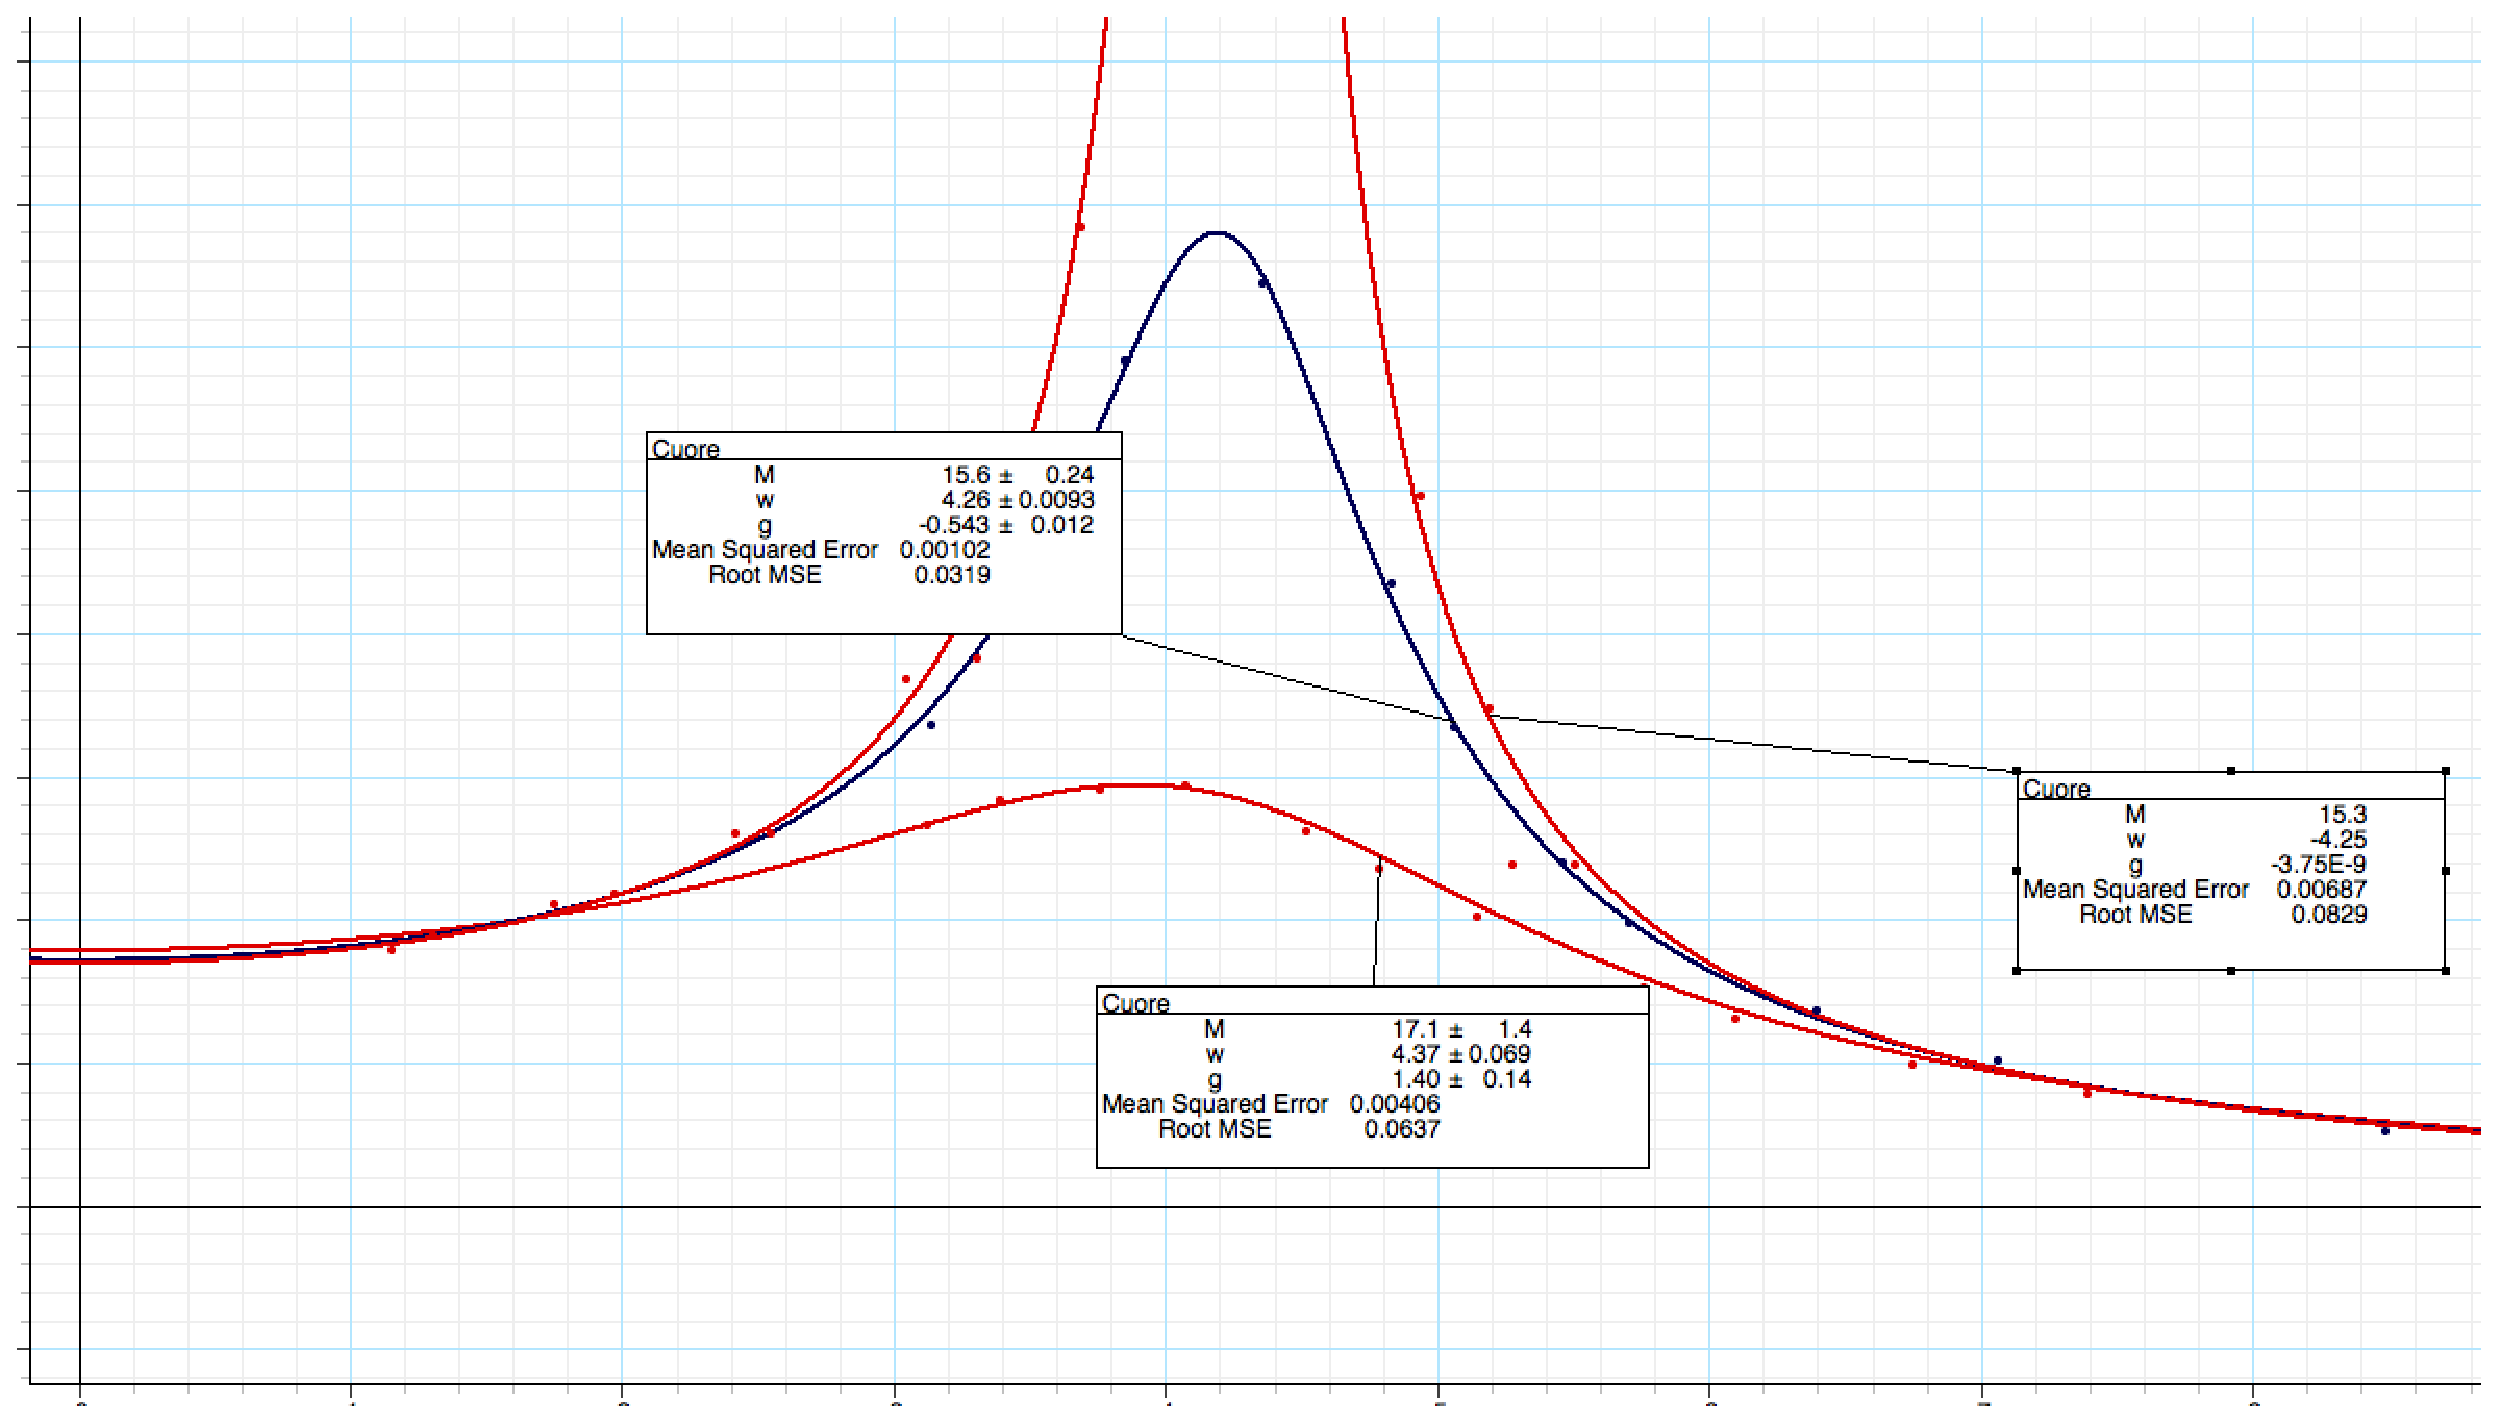
\includegraphics[scale=0.2]{graf}

\section{Conclusioni}
L'esperimento è riuscito un sacco.


\chapter{Bilancia di Cavendish}
\section{Introduzione}
\subsection{Oggetto della ricerca}
Misurazione della costante di gravitazione G mediante la bilancia di Cavendish.
\subsection{Strumenti}
Bilancia di Cavendish\\

\begin{tabular}{ll}
m=38.3$\pm$0.2 g & massa sfere piccole\\
M=1500$\pm$10 g	 & massa sfere grandi\\
r=9.53 mm & raggio sfere piccole\\
R=31.9 mm	 & raggio sfere grandi\\
$m_c\cong 2m$ & massa manubrio\\
\end{tabular}

\subsection{Metodo in breve}
\begin{itemize}
\item a
\end{itemize}
\section{Raccolta dati}
\section{Misura all'equilibrio}
\section{Misura ruotata 180}
\section{Misura periodo}
\section{Analisi dati}
\section{Conclusioni}
\chapter{Banco Ottico}
\section{Introduzione}
\subsection{Scopo dell'esperimento e metodo in breve}
L'esperimento si compone di tre parti.
\\

Nella prima, si verifica la validità della Legge di Snell (vedi contenuti teorici) e la reversibilità del cammino ottico: dato un raggio luminoso attraversante un semi-cilindro in plexiglass, misuriamo l'angolo di incidenza $\theta_{rifrazione}$ ed il corrispondente  angolo di rifrazione $\theta_{rifrazione}$. Sempre grazie alla legge di Snell si ricerca la miglior stima dell'indice di rifrazione del plexiglass $n$.
\\

Nella seconda parte, si ricerca $n$ studiando l'angolo di deviazione minima $\delta_{min}$ di un prisma a base triangolare e di un prisma a base trapezoidale (vedi contenuti teorici). 
Inoltre, si ricerca la distanza di cui viene traslato il raggio, che arriva con un certo angolo di incidenza $\theta$, quando passa per due superfici parallele.
\\

Infine si verifica la legge dei punti coniugati tramite la misura delle distanze $p$ e $q$ e la validità dell'ingrandimento ottico M. 

\subsection{Strumenti}
In questa tabella vengono riassunti gli strumenti rivelatori utilizzati, con le relative precisioni, e il set-up dell'esperimento.\\
\begin{center}
\begin{tabular}{c|c}
Strumento & Precisione \\
\midrule
Piatt. Graduata & $\pm 1 grado $ \\
Metro & $\pm 1 mm $\\
\end{tabular}
\end{center}


Durante l'esperimento è stato impostato sulla modalità a singolo raggio luminoso per le prime due parti e successivamente sulla modalità oggetto per la terza e ultima parte. 
Questo proiettore, insieme alla piattaforma girevole graduata, alle lenti ed a uno schermo bianco, può scorrere liberamente lungo una rotaia, permettendo di modificare le distanze tra gli oggetti a piacimento.

\section{Reversibilità del cammino luminoso}
\subsection{Raccolta dati}
Tutte le misure seguenti sono espresse in gradi.\\
\begin{center}

\begin{tabular}{c|c||c|c}
 \multicolumn{2}{c}{\textit{Faccia piana}} &
\multicolumn{2}{c}{\textit{Faccia curva}} \\
$\theta_{incidenza} $ & $\theta_{rifrazione} $ &$\theta_{incidenza} $ & $\theta_{rifrazione} $\\
\midrule
 10 & 7 & 7 & 10 \\
15 & 10 & &\\
20 & \textbf{13.5} & 13.5 & 20\\ 
25 & \textbf{16.5} & & \\
30 & 20 & 30 & 20\\
40 & 26 & 26 & 40\\
35 & 23 & &\\
45&  \textbf{28.5} & & \\
\multicolumn{4}{c}{\textit{Misure in gradi}} \\
\end{tabular}
\end{center}

\subsection{Analisi dei dati}
Raccolti i valori degli angoli di incidenza e dei corrispondenti angoli di rifrazione, possiamo calcolare la miglior stima di $n$. 
La legge di Snell esprime la relazione che lega gli indici di rifrazione dei due materiali attraversati dal raggio luminoso, e i seni degli angoli di incidenza e rifrazione:\\

\begin{center}
$n_1 sin\theta_1 = n_2 sin\theta_2$
\end{center}

Poiché $n_a \simeq1 $ ( indice di rifrazione dell'aria ), si ricava:

$$n_2 = \frac{sin\theta_1}{sin\theta_2}$$

Nell'elaborazione dei dati, abbiamo selezionato solo le coppie di misure cui corrispondesse un errore relativo percentuale minore del 6\%, al fine di avere una stima più precisa del valore vero di $n$.\\
\begin{center}


\begin{tabular}{c|c|c|c|c|c}
\textbf{$\theta_1$} & 25 & 30 & 40 & 35 & 45\\
\midrule
\textbf{$\theta_2$} & 16.5 & 20 & 26 & 23 & 28.5\\
\midrule
\textbf{$n_i$} (*) & 1.489 & 1.462 & 1.468 & 1.468 & 1.482\\
\end{tabular}\\

\end{center}
(*) in questo caso abbiamo tenuto un numero superiore di cifre significative, in quanto si tratta di calcoli intermedi

$$\overline{n} = \frac{\displaystyle\sum\limits_{i=1}^N n_i}{N} = 1.47$$

$$\sigma_n = \sqrt{\frac{\displaystyle\sum\limits_{i=1}^N n_i}{N-1}} = 0.01$$

$$\sigma_{\overline{n}} = \frac{\sigma_n}{\sqrt{N}} = 0.004$$

$$n_{best} = 1.47 \pm 0.004 $$

\section{Misura dell'angolo di deviazione minima}
\subsection{Raccolta dati}
\subsection{Analisi dei dati}

\section{Lenti sottili}
A destra, misure con lente di focale $f=100 mm$, a sinistra misure con lente di focale $f=200mm$ 
\\
\begin{center}
\begin{tabular}{c|c|c||c|c|c}
p($cm$) &q($cm$)&d($cm$) &p($cm$) &q($cm$)&d($cm$)\\
\midrule
13.5 & 36.5 & 5.5 & 73.4 & 26.6 & 0.7\\
36.2 & 13.8 & 0.8 & 26.4 & 73.6 & 5.5\\
\midrule
18.0 & 22.0 & 2.5 & 61.5 & 28.5 & 0.9\\
22.0 & 18.0 & 2.1 & 28.1 & 61.9 & 4.8\\
\end{tabular}
\end{center}
\subsection{Raccolta dati}
\subsection{Analisi dei dati}

\section{Conclusioni}

\chapter{Pendolo di Kater}
\section{Introduzione}
\subsection{Scopo dell'esperimento}
Misura di g
\subsection{Metodo}
\subsection{Strumenti}
Pendolo di Kater (struttura definita in seguito)
$d(m_a,c_1)=15.4 cm$
Cronometro digitale con fotocellula $\pm 0.0001 s$ 
\section{Raccolta Dati}
\begin{tabular}{| c | c | c | c | c | c | c |}

\textbf{$d(m_b,c_1)=15cm$} & \textbf{$d(m_b,c_1)=17.9cm$} & \textbf{$d(m_b,c_1)=84.4cm$}& \textbf{$d(m_b,c_1)=81.3cm$}& \textbf{$d(m_b,c_1)=12cm$}\\
\midrule
 \textbf{Coltello1}&\textbf{Coltello1}&\textbf{Coltello1}&\textbf{Coltello1}&\textbf{Coltello1}&\textbf{Coltello1}&\textbf{Coltello1}\\
 1.9809 & 1.9211 & 1.9934 & 1.9735 & 2.0040\\
 1.9796 & 1.9207 & 1.9932 & 1.9744 & 2.0041\\
 1.9816 & 1.9264 & 1.9931 & 1.9746 & 2.0043\\
 1.9794 & 1.9253 & 1.9932 & 1.9755 & 2.0062\\
 1.9821 & 1.9113 & 1.9932 & 1.9765 & 2.0060\\
 1.9805 & 1.9278 & 1.9934 & 1.9769 & 2.0052\\
 1.9802 & 1.9278 & 1.9937 & 1.9770 & 2.0050\\
 1.9804 & 1.9277 & 1.9941 & 1.9760 & 2.0061\\
 1.9810 & 1.9278 & 1.9937 & 1.9754 & 2.0046\\
 1.9831 & 1.9278 & 1.9935 & 1.9750 & 2.0058\\

 \textbf{Coltello2}&\textbf{Coltello2}&\textbf{Coltello2}&\textbf{Coltello2}\\
 1.9934 & 1.9882 & 1.9946 &	1.9802 & \\
 1.9946 & 1.9902 & 1.9939 &	1.9812\\
 1.9911 & 1.9907 & 1.9943 &	1.9820\\
 1.9919 & 1.9908 & 1.9941 &	1.9818\\
 1.9940 & 1.9907 & 1.9940 &	1.9819\\
 1.9923 & 1.9907 & 1.9952 &	1.9813\\
 1.9939 & 1.9888 & 1.9954 &	1.9816\\
 1.9934 & 1.9898 & 1.9943 &	1.9818\\
 1.9914 & 1.9898 & 1.9947 &	1.9812\\
 1.9958 & 1.9878 & 1.9941 &	1.9810\\
 
 
\end{tabular}

Abbiamo ricavato i seguenti valore medi e dev.standard 
\begin{tabular}{|c|c|c|}
$d(m_b,c_1)$ & Periodo in c1 & $\sigma$ \\
\midrule
6.9 & 2.1108 &\\
11.7 & 2.0075 &\\
13.5 & &\\
15.0 &  1.9806 &\\
17.9 & 1.9244 &\\
21.0 & 1.9076 &\\
81.3 & 1.9755&\\
84.4 & 1.9935&\\
\end{tabular}

\begin{tabular}{|c|c|c|}
$d(m_b,c_1)$ & Periodo in c2 & $\sigma$ \\
\midrule
6.9 & 2.1108 &\\
11.7 & 2.0075 &\\
13.5 & &\\
15.0 &  1.9806 &\\
17.9 & 1.9244 &\\
21.0 & 1.9076 &\\
81.3 & 1.9755&\\
84.4 & 1.9935&\\
\end{tabular}

$\pm\sigma$

\end{document} 



